\chapter{Rational Functions and Their Graphs}

\section{Domain, Vertical Asymptotes, and Holes}

Much of these concepts boils down to factoring the numerator and denominator \textbf{completely}.

\subsection*{Domain}

For the domain, find the values of $x$ that cause the denominator to equal 0. \\

\begin{example} 
State the domain of
\[
f(x) = \frac{2x^3 + 5x^2 - 3x}{5x^2 + 17x + 6}
\]
\end{example}

\begin{solution}
We want to find the values of $x$ that cause the denominator to equal 0 and \underline{avoid those values}.

\begin{align*}
    5x^2 + 17x + 6 &\neq 0  \\
    (5x + 2)(x + 3) &\neq 0 \qquad 5x^2 + 17x + 6 \text{ factors as } (5x+2)(x+3) \\
    5x + 2 \neq 0 &\text{ and } x + 3 \neq 0 \qquad \text{set each factor } \neq 0 \\
    x \neq -\tfrac{2}{5} &\text{ and } x \neq -3 \\
\end{align*}

So the domain of the answer is $x \neq -\tfrac{2}{5}$ and $x \neq -3$.
\end{solution}

\subsection*{Vertical Asymptotes and Holes}

At each of these domain values, there is either a {\color{red}\textbf{vertical asymptote}} or a {\color{red}\textbf{hole in the graph}}.    \\

In order to know which each value is, we need to factor the numerator as well and simplify our expression. \\

\begin{example}
Simplify 
\[
f(x) = \frac{2x^3 + 5x^2 - 3x}{5x^2 + 17x + 6}
\]
\end{example}

\begin{solution}
\begin{align*}
    \frac{2x^3 + 5x^2 - 3x}{5x^2 + 17x + 6} &= \frac{x(2x^2 + 5x - 3)}{(5x+2)(x-3)} \qquad \text{Factor $x$ out of numerator as a GCF.} \\[6pt]
    &= \frac{x(2x-1)(x+3)}{(5x+2)(x+3)} \qquad 2x^2 + 5x - 3 = (2x-1)(x+3) \\[6pt]
    &= \frac{x(2x-1)}{5x+2} \qquad \text{The $x+3$ terms divide out to 1} \\
\end{align*}
\end{solution}

Now, we are going to take each of those domain values of $x$ ($-\tfrac{2}{5}$ and $-3$) and evaluate the simplified expression $\frac{x(2x-1)}{5x+2}$

\begin{itemize}
    \item If we get an error message (like \textit{undef}), then that value of $x$ is a \textbf{vertical asymptote}.
    \item If we get an actual number back, then that value of $x$ is a \textbf{hole} in the graph. The $y$-coordinate of the hole in the graph is the number we got back.
\end{itemize}


\begin{example}
Evaluate $\frac{x(2x-1)}{5x+2}$ for $x = -\tfrac{2}{5}$ and $x = -3$. 
\end{example}

\begin{solution}

When $x = -\tfrac{2}{5}$, we get
\[
\frac{-\tfrac{2}{5}\left(2(-\tfrac{2}{5})-1\right)}{5\left(-\tfrac{2}{5}\right)+2} = \text{undefined}
\]

When $x = -3$, we get
\[
\frac{-3(2(-3)-1)}{5(-3)+2} = -\frac{21}{13}
\]

Thus, $x = -\tfrac{2}{5}$ is the equation of a vertical asymptote, and there is a hole in the graph at $\left(-3, -\tfrac{21}{13}\right)$
\end{solution}

%{\color{red}{\color{red}\textbf{Exercise.}}} State the domain of each. Then determine the exact coordinates of any holes in the graph and any equations of vertical asymptotes.
%
%\begin{multicols}{3}
%\begin{enumerate}[(a)]
%    \item $f(x) = \frac{3x^2 - x - 10}{x^2 + 5x - 14}$
%    \item $g(x) = \frac{2x^3 + 5x^2 - 3x}{10x^2 + 3x - 4}$
%    \item $h(x) = \frac{3x^2 - 19x - 14}{4x^3 - 24x^2 - 108x}$
%\end{enumerate}
%\end{multicols}

%%%%%%%%%%%%%%%%%%%%%%%%%%%%%%%%%%%%%%%%%%%%%%%%%%%%%%%%%%%%%%%%%%
\iffalse 

(a) 
Domain: $x \neq -7, 2$
Hole @ (2, 11/9)
Vertical asymptote: $x = -7$

(b)
Domain: $x \neq 1/2, -4/5$
Hole @ (1/2, 7/26)
Vertical asymptote: $x = -4/5$

(c)
Domain: $x \neq 0, -3, 9$
No holes
Vertical asymptotes: $x = 0$, $x = -3$, $x = 9$

\fi 
%%%%%%%%%%%%%%%%%%%%%%%%%%%%%%%%%%%%%%%%%%%%%%%%%%%%%%%%%%%%%%%%%%

\section{End Behavior}

End behavior has nothing to do with domain. \newline

So anything from the previous part is not going to help here. \newline 

Instead, end behavior focuses on the behavior of the function as $x$ approaches $-\infty$ and $x$ approaches $\infty$. \newline 

You will want to focus on the \emph{degrees} of the numerator and denominator. \newline 

For rational functions, each function will fall into one of the following three cases.

\begin{center}
\begin{tabular}{l|l}
\textbf{The bigger degree is} & \textbf{End Behavior} \\ \hline
In the denominator & $y = 0$    \\
Degrees are equal   & $y = $ ratio of leading coefficients \\
In the numerator    & $y = $ use polynomial division (up to you get the constant) \\
\end{tabular}
\end{center}

\vspace{12pt}

\begin{example}
Find the end behavior asymptote for each.

\begin{multicols}{3}
\begin{enumerate}[(a)]
    \item $f(x) = \frac{3x+1}{2x^2-5x-3}$
    \item $g(x) = \frac{x^3 - 4x^2 + 7}{5x^3 + 3x}$
    \item $h(x) = \frac{x^3+2x^2-15x}{x^2-5x-14}$
\end{enumerate}
\end{multicols}
\end{example}

\begin{solution}

(a) The bigger degree is in the denominator. Thus, the end behavior is $y = 0$. \newline 

(b) The degrees are equal (both are 3). Thus, the end behavior is the ratio of leading coefficients: $y = \frac{1}{5}$. \newline 

(c) The bigger degree is in the numerator, so you will need to use polynomial division. \newline 

The good news is, you don't need to complete the polynomial division. You only need to stop once you get the constant of the quotient; the remainder approaches 0 as $x \to -\infty$ and $x \to \infty$.

\[
\left(x^3 + 2x^2 - 15x\right) \div \left(x^2 - 5x - 14\right)
\]

\begin{center}
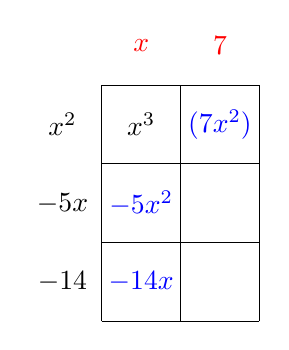
\begin{tikzpicture}
\draw (0,0) grid (2, 3);
\node at (0.5, 2.5) {$x^3$};
\node at (-0.5, 2.5) {$x^2$};
\node at (-0.5, 1.5) {$-5x$};
\node at (-0.5, 0.5) {$-14$};
\node at (0.5, 3.5) [color = red] {$x$};
\node at (0.5, 1.5) [color = blue] {$-5x^2$};
\node at (0.5, 0.5) [color = blue] {$-14x$};
\node at (1.5, 2.5) [color = blue] {$(7x^2)$};
\node at (1.5, 3.5) [color = red] {$7$};
\end{tikzpicture}
\end{center}

Thus, the end behavior asymptote is $y = x + 7$. \newline 
\end{solution}

%{\color{red}{\color{red}\textbf{Exercise.}}} Find the end behavior asymptote for each.
%
%\begin{multicols}{3}
%\begin{enumerate}[(a)]
%    \item $f(x) = \frac{3x^2 - x - 10}{x^2 + 5x - 14}$
%    \item $g(x) = \frac{2x^3 + 5x^2 - 3 x}{10x^2 + 3x - 4}$
%    \item $h(x) = \frac{3x^2 - 19x - 14}{4x^3 - 24x^2 - 108x}$
%\end{enumerate}
%\end{multicols}

%%%%%%%%%%%%%%%%%%%%%%%%%%%%%%%%%%%%%%%%%%%%%%%%%%%%%%%%%%%%%%%%%%
\iffalse 

(a) y = 3
(b) y = (1/5)x + 11/25
(c) y = 0

\fi

\section{Exercises}

Find the domain, coordinates of any holes, and equations of all asymptotes.
\begin{multicols}{2}
\begin{enumerate}
\setlength\itemsep{10pt}
	\item $f(x) = \frac{2x^2+5x-3}{2x^2-15x+7}$
	\item $g(x) = \frac{3x^3+7x^2-20x}{x^2-x-12}$
\end{enumerate} \setcounter{Review}{\value{enumi}}
\end{multicols}
\begin{multicols}{2}
\begin{enumerate}	\setcounter{enumi}{\value{Review}}
	\item $f(x) = \frac{3x}{x+4}$
	\item $g(x) = \frac{x^2+3x+2}{x-1}$
\end{enumerate} \setcounter{Review}{\value{enumi}}
\end{multicols}
\begin{multicols}{2}
\begin{enumerate}	\setcounter{enumi}{\value{Review}}
	\item $h(x) = \frac{x^2+3x-4}{x^3-2x^2+x}$
	\item $f(x) = \frac{2x^3-13x^2+6x+45}{x^2-4x-5}$
\end{enumerate} \setcounter{Review}{\value{enumi}}
\end{multicols}
\begin{multicols}{2}
\begin{enumerate}	\setcounter{enumi}{\value{Review}}
	\item $g(x) = \frac{5x^2-19x-4}{x^3+2x^2-24x}$
	\item $h(x) = \frac{2x^2-x-3}{8x^2+51x+18}$
\end{enumerate} \setcounter{Review}{\value{enumi}}
\end{multicols}
\begin{multicols}{2}
\begin{enumerate}	\setcounter{enumi}{\value{Review}}
	\item $f(x) = \frac{6x^3 - 21x^2 - 51x + 30}{3x^2+7x+2}$
	\item $g(x) = \frac{10x^2-29x-21}{10x^3-33x^2-7x}$
\end{enumerate} \setcounter{Review}{\value{enumi}}
\end{multicols}
\begin{multicols}{2}
\begin{enumerate}	\setcounter{enumi}{\value{Review}}
	\item $f(x) = \frac{x^3+x^2-6x}{3x^2-3x-6}$
	\item $f(x) = \frac{x^2-4x+3}{2x^2+2x-12}$
\end{enumerate} \setcounter{Review}{\value{enumi}}
\end{multicols}
\begin{multicols}{2}
\begin{enumerate}	\setcounter{enumi}{\value{Review}}
	\item $f(x) = \frac{x-4}{-2x^2+4x+16}$
	\item $f(x) = \frac{x^3-2x^2-8x}{x^3-2x^2-3x}$
\end{enumerate} \setcounter{Review}{\value{enumi}}
\end{multicols}
\begin{multicols}{2}
\begin{enumerate}	\setcounter{enumi}{\value{Review}}
	\item $f(x) = \frac{x^2+x-2}{3x^2+3x-18}$
	\item $f(x) = \frac{x^2-3x+2}{4x^2-12x}$
\end{enumerate}	\setcounter{Review}{\value{enumi}}
\end{multicols}
\begin{multicols}{2}
\begin{enumerate}	\setcounter{enumi}{\value{Review}}
	\item $f(x) = \frac{8x^2+26x+15}{2x^2-x-15}$
	\item $g(x) = \frac{x^2-1}{2+2x}$
\end{enumerate}	\setcounter{Review}{\value{enumi}}
\end{multicols}
\begin{multicols}{2}
\begin{enumerate}	\setcounter{enumi}{\value{Review}}
	\item $f(x) = \frac{10x^2 + 28x - 6}{12x^2+45x+27}$
	\item $g(x) = \frac{x-5}{x^2-7x+10}$
\end{enumerate}	\setcounter{Review}{\value{enumi}}
\end{multicols}
\begin{multicols}{2}
\begin{enumerate}	\setcounter{enumi}{\value{Review}}
	\item $h(x) = \frac{2x^3-5x^2-42x}{3x-18}$
\end{enumerate}	\setcounter{Review}{\value{enumi}}
\end{multicols}
\vspace{0.25in}

State the end behavior of each.
\begin{enumerate}	\setcounter{enumi}{\value{Review}}
	\item $k(x) = \frac{5x^3-7x^2+8}{-3x^3+6x-4}$
	\item $m(x) = \frac{2x-1}{3x^2+7x+1}$
\end{enumerate}	\setcounter{Review}{\value{enumi}}

%%%%%%%%%%%%%%%%%%%%%%%%%%%%%%%%%%%%%%%%%%%

Answer each of the following given $h(x) = \frac{6x^3+40x^2-14x}{3x^2+11x-4}$
\begin{enumerate}	\setcounter{enumi}{\value{Review}}
	\item End behavior
	\item Domain of $h$
	\item Equation(s) for any vertical asymptotes
	\item Exact coordinates of any holes
	\item What is the approximate value of $h\!\left(5^{933}\right)$?
\end{enumerate}	\setcounter{Review}{\value{enumi}}

\newpage

\section{Answer Key}

\begin{enumerate}
    \item Domain: $x \neq \frac{1}{2}, \, 7$; V.A.: $x=\frac{1}{2}, \, x=7$; H.A.: $y=1$
    \item Domain: $x \neq -3, \, 4$; V.A.: $x=-3 \, x = 4$; Obl. Asymp: $y = 3x+10$
    \item Domain: $x \neq -4$; V.A.: $x = -4$; H.A.: $y = 3$
    \item Domain: $x \neq 1$; V.A.: $x = 1$; Obl. Asymp: $y = x + 4$
    \item Domain: $x \neq 0, 1$; V.A.: $x = 0$ and $x = 1$; H.A.: $y = 0$ 
    \item Domain: $x \neq -1, 5$; V.A. $x=-1$; Hole @ $\left(5, \frac{13}{3}\right)$; Obl. Asym $y = 2x-5$
    \item Domain: $x \neq -6, 0, 4$; V.A. $x = -6, \, x = 0$; Hole @ $\left(4, \frac{21}{40}\right)$; H.A. $y = 0$
    \item Domain: $x \neq -6, -\frac{3}{8}$; V.A. $x = -6, \, x = -\frac{3}{8}$; H.A. $y = \frac{1}{4}$
    \item Domain: $x \neq -2, \, -\frac{1}{3}$; Hole @ $(-2,-21)$; V.A.: $x = -\frac{1}{3}$; Obl. Asymp: $y = 2x-\frac{35}{3}$
    \item Domain: $x \neq -\frac{1}{5}, \, 0, \, \frac{7}{2}$; Hole @ $\left(\frac{7}{2}, \frac{82}{259}\right)$; V.A. $x = -\frac{1}{5}$ and $x=0$; H.A. $y=0$
    \item Domain: $x \neq -1, \, 2$; V.A. $x = -1$; Hole @ $\left(2, \frac{10}{9}\right)$; Obl. Asymp: $y = \frac{1}{3}x+\frac{2}{3}$
    \item Domain: $x \neq -3, \, 2$; V.A. $x = -3$ and $x = 2$; H.A. $y = \frac{1}{2}$
    \item Domain: $x \neq -2, \, 4$; V.A. $x = 2$; Hole @ $\left(4, -\frac{1}{12}\right)$; H.A. $y = 0$
    \item Domain: $x \neq -1, \, 0, \, 3$; V.A. $x = -1$ and $x = 3$; Hole @ $\left(0, \frac{8}{3}\right)$; H.A. $y = 1$
    \item Domain: $x \neq -3, \, 2$; V.A. $x = -3$ and $x = 2$; H.A. $y = \frac{1}{3}$
    \item Domain: $x \neq 0, \, 3$; V.A. $x = 0$ and $x = 3$; H.A. $y = \frac{1}{4}$
    \item Domain: $x \neq -\frac{5}{2}, 3$; V.A. $x = 3$; Hole @ $\left(-\frac{5}{2}, \frac{14}{11}\right)$; H.A. $y = 4$
    \item Domain: $x \neq -1$; No vertical asymptote; Hole @ $(-1,-1)$; Obl. Asymp: $y = \frac{1}{2}x-\frac{1}{2}$
    \item Domain: $x \neq -3, -\frac{3}{4}$; Vert. Asymp: $x = -\frac{3}{4}$; Hole @ $\left(-3, \frac{32}{27}\right)$; Horiz. Asymp: $y = \frac{5}{6}$
    \item Domain: $x \neq 2, 5$; Vert. Asymp: $x = 2$; Hole @ $\left(5, \frac{1}{3}\right)$; Horiz. Asymp: $y = 0$
    \item Domain: $x \neq 6$; Hole @ $\left(6, 38\right)$; Oblique Asymp: $y = \frac{2}{3}x^2 +\frac{7}{3}x$
    
%%%%% End Behavior %%%%%%%%%
    \item $\displaystyle \lim_{x \to -\infty} k(x) = \infty \quad \lim_{x \to \infty} k(x) = -\frac{5}{3}$
    \item $\displaystyle \lim_{x \to -\infty} m(x) = \infty \quad \lim_{x \to \infty} m(x) = 0$
    
    \item $y = 2x + 6$
    \item $x \neq -4, \frac{1}{3}$
    \item $x = -4$
    \item $\left(\frac{1}{3}, \frac{44}{39}\right)$
    \item $2\left(5^{933}\right) + 6$
\end{enumerate}
